
\فصل{مقدمه}

در این فصل مسئله‌ی اصلی پژوهش، یعنی امتیاز ،ASPECT به طور دقیق‌تر مورد بررسی قرار می‌گیرد و علت اهمیت بالای آن در زمینه‌ی سکته‌ی مغزی عنوان می‌شود.
سپس بررسی می‌شود که آیا این مسئله در پژوهش‌ها و محصولات مرتبط، حل شده‌است یا خیر و اینکه پژوهش حاضر چه مزیتی در این حوزه به همراه خواهد داشت.
در پایان نیز ساختار کلی پایان‌نامه شرح داده می‌شود.

\قسمت{تعریف مسئله}

سکته‌ی مغزی یکی از علل مهم مرگ ومیر و ناتوانی‌های اکتسابی در جهان است.
%Donkor, E.S., 2018. Stroke in the century: a snapshot of the burden, epidemiology, and quality of life. Stroke research and treatment, 2018.
امروزه روش‌های درمانی مختلفی برای بیماران مبتلا به این عارضه وجود دارد.
اما تجویز روش درمانی مناسب، برای هر بیمار، با توجه به وضعیت وی، متفاوت است.
در واقع لازم است که متخصصان، ملاک و معیاری از وضعیت پیشرفت و وخامت سکته داشته باشند تا بتوانند یک روش درمانی را برای بیمار، مناسب یا نامناسب قلمداد کنند.
یکی از مهم‌ترین این معیارها، امتیاز ASPECT است.\\

\lr{The Alberta Stroke Program Early CT Score (ASPECTS)} یک امتیاز از ۱ تا ۱۰ است که معیاری از وخامت سکته در بیمار را به دست می‌دهد.
درواقع این امتیاز از بررسی وضعیت ۱۰ ناحیه‌ی مغزی ،که در دو نیم‌کره‌ی مغز به صورت متقارن وجود دارند، محاسبه می‌شود.
شکل ~\ref{fig:aspects-regions} این ۱۰ ناحیه را نشان می‌دهد.
در صورتی که هیچ عارضه‌ی انسدادی در مغز وجود نداشته باشد، امتیاز ASPECT برابر ۱۰ خواهد بود و به ازای هر ناحیه‌ای که آسیب دیده‌است، یک امتیاز از ۱۰ کم می‌شود.
به این ترتیب بیماری که هر ۱۰ ناحیه‌ی ASPECTS او، حداقل در یک نیم‌کره، آسیب دیده‌باشد، امتیاز صفر را دریافت خواهد کرد.

\begin{figure}[ht]
    \centering
    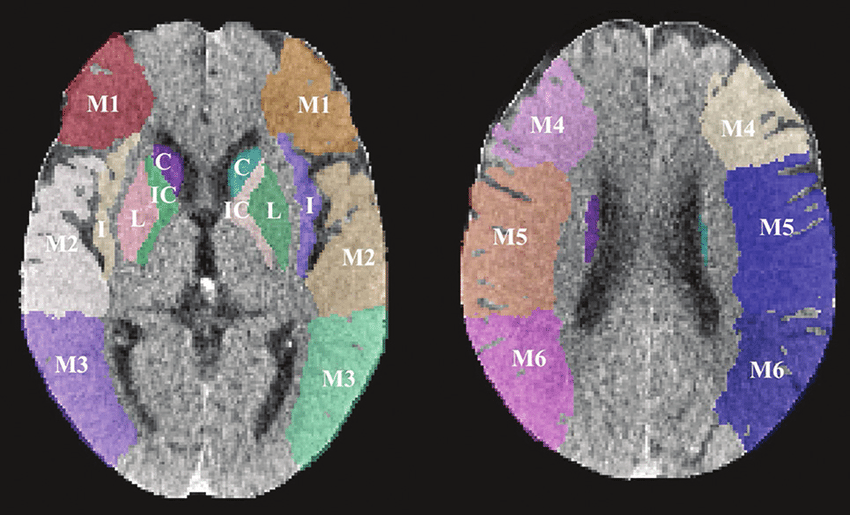
\includegraphics[width=\textwidth, keepaspectratio]{aspects-regions.png}
    \caption[]{نواحی ASPECTS در دو برش از مغز. ۱۰ ناحیه شامل ،I ،C ،L ،IC \lr{M6}-\lr{M1}.}
    \label{fig:aspects-regions}
\end{figure}
%Kuang, Hulin & Najm, Mohamed & Chakraborty, Debabrata & Maraj, Nicholas & Sohn, Sung-Il & Goyal, Mayank & Hill, Michael & Demchuk, Andrew & Menon, Bijoy & Qiu, Wu. (2018). Automated ASPECTS on Non-Contrast CT Scans in Acute Ischemic Stroke Patients Using Machine Learning. American Journal of Neuroradiology. 10.3174/ajnr.A5889. 


این امتیاز سپس می‌تواند معیاری در اختیار متخصصان قرار دهد که تشخیص بدهند آیا لخته‌زدایی مکانیکی
\footnote{\lr{Mechanical Thrombectomy}}
برای بیمار مناسب است یا خیر.
یه عنوان مثال، ممکن است در یک سیاست تصمیم‌گیری، بیمارانی که امتیاز بیشتر/مساوی ۶ را کسب کرده‌اند، برای لخته‌زدایی مکانیکی، مناسب تشخیص داده‌شوند.
% Seyedsaadat, S.M., Neuhaus, A.A., Nicholson, P.J., Polley, E.C., Hilditch, C.A., Mihal, D.C., Krings, T., Benson, J., Mark, I., Kallmes, D.F. and Brinjikji, W., 2021. Differential contribution of ASPECTS regions to clinical outcome after thrombectomy for acute ischemic stroke. American Journal of Neuroradiology, 42(6), pp.1104-1108.
به این نوع از امتیازدهی که وضعیت بیماران را به دو دسته‌ی بالا و پایین یک آستانه تقسیم می‌کنند، امتیاز دوبخشی‌شده‌ی ASPECTS می‌گویند.
درواقع در اکثر موارد، تشخیص درمان لخته‌زدایی به کمک همین حد آستانه بر روی امتیاز ASPECTS انجام می‌شود و از این جهت، به امتیاز‌دهی دوبخشی اهمیت بیشتری می‌بخشد.\\

نکته‌ی حائز اهمیت آن است که امتیازدهی ،ASPECT حتی برای متخصصین این حوزه، یک امر چالش‌بر‌انگیز است.
به نحوی که در یک مطالعه،
%van Horn, N., Kniep, H., Broocks, G., Meyer, L., Flottmann, F., Bechstein, M., Götz, J., Thomalla, G., Bendszus, M., Bonekamp, S. and Pfaff, J.A.R., 2021. ASPECTS interobserver agreement of 100 investigators from the TENSION study. Clinical Neuroradiology, pp.1-8.
میزان توافق میان امتیازدهندگان، تنها ۲۸٪ محاسبه شده‌است.
از طرفی، نشان داده شده‌است که ابزار‌های محاسبه‌ی خودکار ،ASPECT می‌توانند
میزان این توافق و سرعت امتیازدهی متخصصان را افزایش دهند.
%Chen, W., Wu, J., Wei, R., Wu, S., Xia, C., Wang, D., Liu, D., Zheng, L., Zou, T., Li, R. and Qi, X., 2022. Improving the diagnosis of acute ischemic stroke on non-contrast CT using deep learning: a multicenter study. Insights into Imaging, 13(1), pp.1-12.
به همین جهت، این پژوهش قصد دارد با ارائه‌ی یک روش خودکار تشخیص امتیاز دوبخشی ASPECT 
در راستای این بهبود دقت و سرعت، راهگشا باشد.

\قسمت{اهمیت موضوع}
میان دقت، سرعت و دسترس‌پذیری در تشخیص سکته‌ی مغزی، یک بده‌بستان
\footnote{tradeoff}
وجود دارد.
یک‌سری تصاویر مانند ،MRI علائم سکته را بهتر در خود نمایان کرده و تشخیص را برای متخصصان ساده‌تر می‌کنند.
اما اخذ این تصاویر، زمان زیادی نیاز دارد و ممکن است در تمام مراکز تصویر‌برداری نیز در دسترس نباشند.
از سوی دیگر، تصاویر ،CT علائم سکته را کمتر مشخص می‌کنند و باعث می‌شوند که تشخیص، سخت‌تر و توافق میان تشخیص‌دهندگان کمتر شود.
اما مزیت این مدل تصویربرداری، در سرعت اخذ تصویر و کاربرد فراگیر آن در اکثر ماکز تصویر برداری است.\\
اصطلاحی در این حوزه وجود دارد که عنوان می‌کند "زمان، مغز است". 
%Saver, J.L., 2006. Time is brain—quantified. Stroke, 37(1), pp.263-266.
این جمله به اهمیت زمان و لزوم تشخیص و درمان سریع سکته‌ی مغزی اشاره می‌کند.
به طور متوسط، در بیمارانی که دچار سکته‌ی مغزی انسدادی شده‌اند، در هر دقیقه، ۱.۹ میلیون سلول عصبی از بین می‌رود.
این عدد در مقایسه با نرخ عادی از بین رفتن سلول‌های عصبی، مانند آن است که مغز در یک ساعت، به مدت ۳.۶ سال عمر کرده‌است.
%همان
به همین جهت، سرعت عمل در تشخیص سکته‌ی مغزی و آغاز هر چه زودتر درمان آن، امری حیاتی است.
در نتیجه در بده‌بستان میان دقت و سرعت، این سرعت است که برتری می‌یابد و تصویربرداری CT و روش‌های تشخیصی مبتنی بر آن را غالب می‌کند.
امتیازدهی ASPECT یک روش تشخیصی مبتنی بر CT است.
به همین دلیل است که پژوهش حول این مسئله، از اهمیت بالایی برخوردار است.
اما همانطور که پیش‌تر ذکر شد، علی‌رغم سرعت بالای تشخیص در این روش، افزایش دقت حاصل از آن، یک موضوع چالش برانگیز است.
عدم توافق بالا میان تشخیص متخصصان نیز خبر از این مشکل دارد.
مشکلی که همچنان میان متخصصان انسانی ماندگار است.
هوش مصنوعی و روش‌های یادگیری ماشین می‌توانند به حل این مشکل کمک کنند.
پژوهش‌هایی انجام شده‌است
%Chen, W., Wu, J., Wei, R., Wu, S., Xia, C., Wang, D., Liu, D., Zheng, L., Zou, T., Li, R. and Qi, X., 2022. Improving the diagnosis of acute ischemic stroke on non-contrast CT using deep learning: a multicenter study. Insights into Imaging, 13(1), pp.1-12.
که نشان می‌دهد تشخیص خودکار امتیاز ASPECT می‌تواند توافق میان متخصصان را افزایش بدهد.
بنابراین ضروری است که این روش‌ها، با افزایش هرچه بیش‌تر دقت، در راستای بهبود سرعت و دقت خدمات درمانی سکته‌ی مغزی، کمک‌کننده باشند.

\قسمت{ادبیات موضوع}

اکثر دانشگاه‌های معتبر قالب استانداردی برای تهیه‌ی پایان‌نامه در اختیار دانشجویان خود قرار می‌دهند.
این قالب‌ها عموما مبتنی بر نرم‌افزارهای متداول حروف‌چینی نظیر لاتک و مایکروسافت ورد هستند.

 لاتک\پانویس{\LaTeX} یک نرم‌افزار متن‌باز قوی برای حروف‌چینی متون علمی است.\مرجع
 {knuth1984texbook, lamport1985LaTeX} 
در این نوشتار از نرم‌افزار حروف‌چینی زی‌تک\پانویس{\XeTeX} 
 و افزونه‌ی زی‌پرشین\پانویس{\XePersian}
 استفاده شده است.


\قسمت{اهداف پژوهش}

کتابخانه‌ی مرکزی دانشگاه صنعتی شریف دستورالعمل جامعی را در خصوص
نحوه‌ی تهیه‌ی پایان‌نامه‌ی کارشناسی ارشد و رساله‌ی دکتری ارائه کرده است.
در این نوشتار سعی شده است قالب استانداردی برای تهیه‌ی پایان‌نامه‌ها مبتنی بر نرم‌افزار لاتک و
بر اساس دستورالعمل مذکور ارائه شده و
نحوه‌ی استفاده از قالب به طور مختصر توضیح داده شود.
این قالب  می‌تواند برای تهیه‌ی پایان‌نامه‌های کارشناسی و کارشناسی ارشد 
و همچنین رساله‌ها‌ی دکتری مورد استفاده قرار گیرد.

\قسمت{ساختار پایان‌نامه}

این پایان‌نامه در پنج فصل به شرح زیر ارائه می‌شود.
%فصل دوم به بیان مفاهیم اولیه  می‌پردازد.
نکات اولیه‌ی نگارشی و نحوه‌ی نگارش پایان‌نامه در محیط لاتک در  فصل دوم به اختصار اشاره شده است. 
فصل سوم به مطالعه و بررسی کارهای پیشین مرتبط با موضوع این پایان‌نامه می‌پردازد.
در فصل چهارم، نتایج جدیدی که در این پایان‌نامه به‌دست آمده است، ارائه می‌شود.
فصل پنجم به جمع‌بندی کارهای انجام شده در این پژوهش و ارائه‌ی پیشنهادهایی برای انجام کارهای آتی خواهد پرداخت.